\documentclass[conference]{IEEEtran}
\usepackage{amsmath,amssymb}
\usepackage{booktabs}
\usepackage{graphicx}
\usepackage{url}
\usepackage[hidelinks]{hyperref}

\newcommand{\Pzero}{\ensuremath{P_0}}
\newcommand{\Vhat}{\ensuremath{\widehat{V}}}

\begin{document}

\title{Audit-Ready Policy Evaluation for Account-Opening Fraud under Selective and Delayed Labels}

\author{\IEEEauthorblockN{Ken Ira Lacson Talingting}
\IEEEauthorblockA{Independent Researcher\\Philippines\\keniralacson@gmail.com}}

\maketitle

\begin{abstract}
Account-opening fraud policies are evaluated on labels generated by the incumbent policy. Rejected applications are never observed, approved applications are labeled sparsely and late, and a backtest on the labeled rows answers a different question than the one a risk committee asks. We formulate the estimand on the logging non-rejected population, state the identification assumptions, and implement a doubly robust estimator with an identification gate, partial-identification bounds for the reject margin, and a full-policy difference bound with a break-even rejected-fraud rate. On the public BAF benchmark, the naive labeled mean overstates cost by 111.6--278.5\% in the main scenario, and the maximum naive bias across policies is 7.8--538.5\% across a 12-cell observation-rate sweep. The doubly robust estimator has a mean bias of at most 1.89\%, with a 95\% Monte Carlo upper bound of 4.3\% at $e_{\text{approve}}\ge0.05$ and 9.6\% at $e_{\text{approve}}=0.01$, and 84.5--96.0\% coverage; its ranking is correct only 64\% of the time at the lowest label rate, so an accurate point estimate does not imply a correct decision. The ranking failure is cost-dependent: at a false-reject cost of 0.50, the naive rule ranks the true best policy first 100\% of the time while DR does so 58\%, even though the naive point estimate remains biased by 163--291\%. A known-truth test confirms double robustness (+0.14\% with a wrong outcome model, +0.36\% with a wrong propensity); outcome-dependent labels break action-only estimators (up to 1,737\%), while audit-only recovers the logging-approved population; the narrow bounds interval fails a pre-registered coverage gate while the widened interval passes 77 of 88 cells. A reproducible case study shows the naive backtest rejecting a synthetic oracle candidate that is 12.4\% cheaper; the case isolates the evaluation bias, not model-training quality. The results are conditional on a simulated observation mechanism and are not a production estimate. Code, benchmark, and claim checks are released.
\end{abstract}

\begin{IEEEkeywords}
selective labels, off-policy evaluation, doubly robust estimation, delayed feedback, fraud, account opening, model risk
\end{IEEEkeywords}

\section{Introduction}

Every account-opening decision is a choice among approve, review, and reject. The policy that makes the choice also determines which applications are later labeled: reviewed applications are examined, approved applications are labeled only if fraud is reported or a random audit is run, and rejected applications are never observed. A backtest that averages cost over the labeled rows therefore evaluates a selected sample, not the population the policy would face. The selection is not random: reviewed applications are over-represented, and the labels that do arrive are delayed.

The problem is known in two literatures that rarely meet. Work on selective labels studies evaluation when outcomes are observed only for a decision-dependent subset \cite{lakkaraju2017selective,kleinberg2018human}. Reject inference studies how to train a credit model when rejected applicants have no outcome \cite{boyes1989econometric,crook2004reject,ehrhardt2021reject,kozodoi2025fighting,scarone2026illusion}. Off-policy evaluation (OPE) provides doubly robust estimators for logged bandit feedback \cite{dudik2011dr,dudik2014dr,swaminathan2015self,chernozhukov2018dml}. Delayed-feedback work models labels that arrive after the decision \cite{chapelle2014delayed,dalpozzolo2015delayed}. Fraud adds a third feature that the OPE literature usually assumes away: the reject margin is structurally unobserved, so the full-population value is not point-identified from logs alone.

This paper treats the three features together and asks a narrower, testable question: \emph{on the population the incumbent did not reject, what would a candidate policy have cost, and is that estimate identified well enough to support a decision?} We make four contributions.

\begin{enumerate}
\item \textbf{Estimand and identification.} We define the policy value on the logging non-rejected population (\Pzero), state the assumptions, and separate what is identified from what is not. The reject margin is bounded, not estimated.
\item \textbf{A gated estimator.} We combine doubly robust estimation with an identification gate that checks positivity, label counts, effective sample size, weight tails, cost support, the declared observation mechanism, and propensity calibration. The gate refuses a point estimate when the log cannot support one.
\item \textbf{Evidence on what fails.} On the BAF benchmark \cite{jesus2022baf}, we run a 12-cell observation-rate sweep, a propensity and covariate sensitivity, a known-truth double-robustness test, a month-by-month stability check, and a reproducible case study. We report the negative results: outcome-dependent labels break action-only estimators, the narrow bounds interval fails its coverage gate, and we quantify the ranking gap and reject-margin fragility in account-opening. The ranking/selection phenomenon itself is established in the 2026 financial selective-labels work \cite{kuroki2026oscar,bhola2026,hong2026doit}; our contribution is the applied account-opening decision layer, not the phenomenon.
\item \textbf{A decision layer and a reproducible artifact.} The report outputs a paired candidate-vs-incumbent difference, the probability that the candidate is cheaper, the expected regret of each choice, and the labels needed for a target power. Every public number is checked against a committed artifact in CI.
\end{enumerate}

The scope is deliberately limited. The evidence is a simulation on public synthetic data with a normalized cost matrix. We do not claim a production estimate, a causal effect of a live policy change, or that the method generalizes to a specific bank without a partner pilot. The paper's value is the measurement discipline: what can be estimated, what cannot, and what a risk team should do when the log is insufficient. The code, the benchmark, and the claim checks are available at \url{https://github.com/kira-ml/onboarding-audit}.

\section{Related Work}

\subsection{Selective labels and feedback}
Lakkaraju et al.\ formalize the selective-labels problem: a decision policy determines which outcomes are observed, so a model trained or evaluated on observed outcomes inherits the policy's selection \cite{lakkaraju2017selective}. Kleinberg et al.\ show the same mechanism in human decision-making \cite{kleinberg2018human}. Feedback loops make the problem dynamic: today's decisions change tomorrow's training data \cite{ensign2018runaway,perdomo2020performative}, and fraud is a concrete case where the incumbent's review policy shapes the labels \cite{pombal2022prisoners}. Our work is static: we hold the logging policy fixed and evaluate a candidate on the same applications. This is the right scope for a pre-deployment audit, where the question is the value of a policy change, not the long-run equilibrium.

\subsection{Financial selective labels in 2026}
Recent ICAIF 2026 work is closest. OSCAR studies certified online learning for auditable financial screening under selective and delayed labels \cite{kuroki2026oscar}. Beyond Holdout Error proposes a layered evaluation framework and shows that estimator rankings can reverse under selective labels \cite{bhola2026}. DOiT shows that better money-flow ranking can coexist with worse account selection in AML review \cite{hong2026doit}. Adjacent 2026 work applies off-policy evaluation to debt collections \cite{prado2026jubilee} and selection-aware certification to fraud rule portfolios \cite{pande2026selection}; neither targets the account-opening reject margin. These papers establish the ranking/selection problem in finance. Our contribution is the account-opening instantiation: the \Pzero\ estimand, reject-margin bounds and a full-policy break-even, the readiness gate, the audit design, and the open reproducible artifact. We do not claim a new estimator or the ranking phenomenon itself.

\subsection{Reject inference}
Reject inference augments the labeled sample with inferred outcomes for rejected applicants \cite{boyes1989econometric}. The empirical record is mixed: Crook and Banasik find little gain \cite{crook2004reject}; Ehrhardt et al.\ survey the methods and their assumptions \cite{ehrhardt2021reject}; Kozodoi et al.\ frame sampling bias as a training and evaluation problem \cite{kozodoi2025fighting}; Scarone and Baeza-Yates warn that apparent improvements can be artifacts \cite{scarone2026illusion}. Our target is different. We do not infer rejected outcomes; we estimate the value on the non-rejected population and bound the reject margin. This avoids a model for the unobservable and makes the limitation explicit.

\subsection{Off-policy evaluation}
Doubly robust (DR) estimation combines an outcome model with inverse propensity weighting and is consistent if either is correct \cite{dudik2011dr,dudik2014dr}. The self-normalized estimator reduces weight variance \cite{swaminathan2015self}, and double/debiased machine learning provides the cross-fitting and inference framework \cite{chernozhukov2018dml}. Positivity diagnostics are standard in causal inference \cite{petersen2012positivity}; unobserved confounding is a known limit \cite{namkoong2020unobserved}. We apply these tools to a fraud log where the propensity is action-level or covariate-dependent, and we test the double-robustness property directly rather than asserting it.

\subsection{Delayed feedback and fraud metrics}
Delayed feedback is modeled explicitly in display advertising \cite{chapelle2014delayed} and in credit-card fraud with concept drift \cite{dalpozzolo2015delayed}. Fraud evaluation also has domain metrics such as value detection rate \cite{dervovic2023vdr}. We use a cost matrix rather than a ranking metric, because the decision is a capacity-constrained choice among actions, and we model label delay as a resolution probability.

\subsection{Positioning}
The closest work is the 2026 financial selective-labels work above \cite{kuroki2026oscar,bhola2026,hong2026doit}; the established credit-scoring literature studies sampling bias \cite{kozodoi2025fighting,scarone2026illusion}, and generic OPE assumes logged rewards. This paper's contribution is the applied combination: a \Pzero\ estimand, a readiness gate that refuses unidentified logs, partial-identification bounds for the reject margin, a full-policy break-even, an audit design, and an open reproducible artifact. The ranking/selection gap is established; we quantify it in account-opening and add the reject-margin decision layer.

\section{Problem Formulation}

\subsection{Notation}
Let $i=1,\dots,n$ index applications. Let $A_i\in\{\text{approve},\text{review},\text{reject}\}$ be the logging action, $X_i$ pre-decision covariates, $Y_i\in\{0,1\}$ fraud, and $C(a,Y_i,m_i)$ the cost of action $a$ with credit-line exposure $m_i$. The cost matrix has four parameters: fraud loss rate, review cost, false-reject cost, and residual fraud loss. It is an assumption, not a measurement.

\subsection{Estimand}
The primary estimand is the mean cost of a candidate policy $\pi$ on the logging non-rejected population
\begin{equation}
V_{\Pzero}(\pi)=\mathbb{E}\left[C(\pi(X),Y,m)\mid A\neq\text{reject}\right].
\end{equation}
The candidate may take a different action than the log, but $Y$ is a property of the application, not of the action. The reject margin is outside the estimand: for $A=\text{reject}$, $Y$ is never observed.

\subsection{Identification}
$V_{\Pzero}$ is identified under seven assumptions: (i) consistency, the observed label is the application's fraud status; (ii) positivity, $e_i=\Pr(R_i=1\mid A_i,X_i)>0$ on \Pzero, where $R_i$ indicates observation; (iii) no unmeasured confounding of observation, $R\perp Y\mid A,X$; (iv) a correct or consistently estimated observation model; (v) a stable cost model; (vi) no interference; and (vii) action-invariant outcome, the action does not change $Y$. Assumption (iii) fails when approved fraud is more likely to be reported than approved legitimate behavior. The gate cannot test it; the analyst must declare it, and an audit is the fallback.

\subsection{Why the reject margin is not identified}
For a rejected application, the candidate action's cost is bounded by the cost model: approve costs in $[0,\text{fraud loss}]$, review in $[\text{review cost},\text{review cost}+\text{residual}]$, and reject in $[0,\text{false-reject cost}]$. The mean over rejected rows therefore lies in an interval, and the full-population value lies in the convex combination of that interval and the \Pzero\ value. A point estimate requires an assumption about the unobserved cost, which we do not make.

\section{Method}

\subsection{Estimators}
Let $w_i=R_i/e_i$ and $n_0=\sum_i\mathbf{1}[A_i\neq\text{reject}]$. The estimators are
\begin{align}
\hat{V}_{\text{naive}}&=\frac{1}{\sum R_i}\sum_{i:R_i=1}C_i,\\
\hat{V}_{\text{HT}}&=\frac{1}{n_0}\sum_i w_i C_i,\\
\hat{V}_{\text{H\'ajek}}&=\frac{\sum_i w_i C_i}{\sum_i w_i},\\
\hat{V}_{\text{DR}}&=\frac{1}{n_0}\sum_i\left[\hat{m}(X_i,\pi)+w_i\left(C_i-\hat{m}(X_i,\pi)\right)\right],
\end{align}
where $C_i$ is the cost under the candidate action computed from the observed $Y_i$, and $\hat{m}(X,\pi)=\mathbb{E}[C(\pi(X),Y,m)\mid X]$ is a cross-fitted outcome model. The influence term for DR is $\psi_i=\hat{m}_i+w_i(C_i-\hat{m}_i)-\hat{V}_{\text{DR}}$, with standard error $\mathrm{sd}(\psi_i)/\sqrt{n_0}$.

\subsection{Double robustness}
Write $m^\ast$ for the true outcome mean and $e^\ast$ for the true propensity. Then
\begin{equation}
\mathbb{E}[\hat{V}_{\text{DR}}]=\mathbb{E}[m]+\mathbb{E}\left[\frac{e^\ast}{e}(m^\ast-m)\right].
\end{equation}
If $m=m^\ast$, the second term is zero for any $e>0$. If $e=e^\ast$, the second term is $\mathbb{E}[m^\ast-m]$, which cancels the first. Hence DR is consistent if either model is correct. The property is a safety net, not a guarantee: when both are wrong, DR is biased.

\subsection{Identification gate}
Before printing a point estimate, the report checks positivity on \Pzero, at least 100 observed labels and 30 per non-rejected action, an effective sample size of at least 100, a maximum weight of at most 100, finite non-negative costs, a declared observation mechanism, and propensity calibration. A declared outcome-dependent mechanism refuses the estimate. An undeclared mechanism marks the memo ``assumption unverified''. A provided propensity with an observed/expected ratio above 1.5 is impossible and refuses; a ratio below 0.5 is flagged as likely too high or heavily censored. The thresholds are conventions, deliberately conservative: a false refusal is cheaper than a confident memo on an unidentified quantity. The gate is a readiness screen, not a test of unmeasured confounding; passing it does not prove the identification assumptions.

\subsection{Bounds}
The conditional interval is
\begin{align}
L(v)&=\frac{n_0}{n}v+\frac{n_{\text{rej}}}{n}\overline{c}_{\min},\\
U(v)&=\frac{n_0}{n}v+\frac{n_{\text{rej}}}{n}\overline{c}_{\max},
\end{align}
where $v$ is the \Pzero\ estimate. It is not a confidence interval. Because $L$ and $U$ are monotone in $v$, a $95\%$ interval for $v$ maps to a valid, conservative interval for the full-population value:
\begin{equation}
\left[L(\hat{v})-1.96\frac{n_0}{n}s_v,\;U(\hat{v})+1.96\frac{n_0}{n}s_v\right].
\end{equation}
The widened interval covers the truth when the \Pzero\ interval does, and it is wider by construction.

\subsection{Decision layer}
For a candidate and the logged policy, the paired DR difference uses $\psi_i^{\text{cand}}-\psi_i^{\text{inc}}$. The report gives the difference, its interval, $P(\text{candidate cheaper})=\Phi(-\Delta/\mathrm{se})$, and the expected regret of each choice, $\mathbb{E}[\max(0,\Delta)]$ and $\mathbb{E}[\max(0,-\Delta)]$ under a normal approximation. It also reports the labels needed for $80\%$ power to detect a $5\%$ and $10\%$ difference, $n_0(z_{0.975}+z_{0.8})^2(\mathrm{se}/\delta)^2$, as a planning approximation.

The paired comparison is \Pzero-conditional. To keep a \Pzero\ recommendation from being read as a full-policy decision, we bound the candidate-vs-incumbent difference directly. For each logging-rejected row $i$, let $d_i(y)=C(\pi_c(X_i),y,m_i)-C(\pi_0(X_i),y,m_i)$ for $y\in\{0,1\}$. The mean reject-margin difference lies in $[\overline{\min(d_i(0),d_i(1))},\overline{\max(d_i(0),d_i(1))}]$, and the full difference lies in
\begin{equation}
\begin{aligned}
L &= \frac{n_0}{n}\left(\Delta - z\,\mathrm{se}_\Delta\right)
+\frac{n_{\text{rej}}}{n}\overline{\min\{d_i(0),d_i(1)\}},\\
U &= \frac{n_0}{n}\left(\Delta + z\,\mathrm{se}_\Delta\right)
+\frac{n_{\text{rej}}}{n}\overline{\max\{d_i(0),d_i(1)\}}.
\end{aligned}
\end{equation}
This is sharper than differencing two separate policy bounds because the same application's outcome is shared by both policies. If the interval excludes zero, the direction survives any reject outcome. If it does not, we report the break-even fraud rate $p^\ast$ under a common-rate assumption, $D_{\text{full}}(p)=0$; a \Pzero\ recommendation that does not survive the reject margin is flagged. The break-even is a sensitivity threshold, not an estimate.

\section{Experimental Design}

\subsection{Data}
We use the Bank Account Fraud (BAF) benchmark \cite{jesus2022baf}, a public synthetic account-opening dataset generated from an anonymized real portfolio. The evaluation window is months 5--6 (227,491 applications, 1.2576\% fraud). The policy scores are trained on months 0--2 with fixed hyperparameters; months 3--4 are held out from evaluation but are not used for hyperparameter selection in this reproduction. The nuisance outcome model is cross-fitted on the evaluation window's observed labels; the candidate policy's labels are not used to fit the policy scores. The processed frame is rebuilt from the public \texttt{Base.csv} and reproduced the recorded SHA-256 exactly.

\subsection{Observation mechanism}
The log is simulated with an action-dependent observation probability: reviewed applications resolve with probability $\kappa_{\text{review}}$, approved applications with a post-approval report probability plus a random audit, and rejected applications are never observed. Labels resolve with a delay (45-day median for approvals), and the cutoff is 90 days. The main scenario uses $e_{\text{approve}}=0.05$ (a pre-resolution report probability; 3.06\% realized), $\kappa_{\text{review}}=0.90$, and a 1\% audit. The cost matrix is normalized: fraud loss $m\cdot0.0019187869$, review cost 0.02, false-reject cost 0.10, residual fraud loss 0.30. The fraud-loss normalizer is $1/\overline{m}$ on the training window, so the mean fraud loss is one cost unit.

\subsection{Scenarios}
The main scenario uses 100 replications. The observation-rate sweep crosses $e_{\text{approve}}\in\{0.01,0.05,0.20,0.50\}$ with $\kappa_{\text{review}}\in\{0.50,0.90,1.00\}$ (12 cells, 50 replications each). The sensitivity study replaces the oracle propensity with an estimated action-level rate, lognormal noise ($\sigma=0.10,0.25$), and outcome-dependent labels; it also compares action-level, fitted covariate, and oracle propensities under covariate-dependent observation. The double-robustness test uses a separate semi-synthetic outcome with a known interaction (200 replications). The temporal check re-runs the main scenario on months 5 and 6 separately (100 replications each). The case study is a committed 20,000-row synthetic log with a known truth.

\subsection{Metrics}
We report relative bias, coverage of the $95\%$ interval, effective sample size (ESS), maximum weight, pairwise rank inversions, the probability of selecting the true best policy, the cost of misranking, and bounds width. Coverage is a diagnostic, not a guarantee: heavy weights can undercover even when the point estimate is close. Monte Carlo uncertainty is reported as $\mathrm{sd}(\text{estimate})/\sqrt{\text{reps}}$; the $95\%$ bound on $|\text{bias}|$ is $|\text{mean bias}|+1.96\,\mathrm{mc\_se}$.

\section{Results}

\subsection{Naive bias and rank reversal}
Table~\ref{tab:main} reports the main scenario. The naive labeled mean overstates cost by 111.6--278.5\%, and it reverses the ranking: it puts the incumbent ahead of the better model, while the true ranking is the opposite. The mean number of pairwise inversions is 1.00, and the naive rule selects the true best policy in 0\% of replications. The direction is not universal in sign; it depends on which action dominates the labeled sample.

\begin{table}[t]
\centering
\caption{Main scenario: true \Pzero\ cost, naive estimate, and DR estimate. Coverage is the share of $95\%$ intervals containing the truth.}
\label{tab:main}
\footnotesize
\begin{tabular}{lrrrrr}
\toprule
Policy & True & Naive & Naive bias & DR & Cov.\\
\midrule
Incumbent & .00879 & .01858 & +111.6\% & .00870 & 95\%\\
Better model & .00845 & .02584 & +205.7\% & .00837 & 96\%\\
Strict cost & .01276 & .03851 & +201.8\% & .01272 & 97\%\\
Lenient cost & .00954 & .03611 & +278.5\% & .00948 & 96\%\\
\bottomrule
\end{tabular}
\end{table}

\subsection{DR recovery and its limits}
DR has a mean bias of at most 0.94\% in the main scenario and 96.0\% coverage. IPW is at 1.18\% and 94.5\%. The ranking is better but not perfect: DR mean inversions 0.29 and $P(\text{best})=72\%$. The point estimate and the ranking are different objects, and the paper reports both.

\subsection{Observation-rate sweep}
Fig.~\ref{fig:sweep} and Table~\ref{tab:sweep} show the sweep. The maximum naive bias across policies is 7.8--538.5\% and exceeds 5\% in 12/12 cells; the incumbent's own bias is 1.5--218\% and exceeds 5\% in 11/12. DR's mean bias is at most 1.89\%; its $95\%$ Monte Carlo upper bound is 4.3\% for $e\ge0.05$ and 9.6\% at $e=0.01$. Coverage is 84.5--96.0\%. At the lowest report probability, DR selects the true best policy 64\% of the time (95\% Wilson interval [50\%, 76\%]); the naive rule does so 0\% of the time. The direction of the contrast is solid; the decimal places are not.

\begin{figure}[t]
\centering
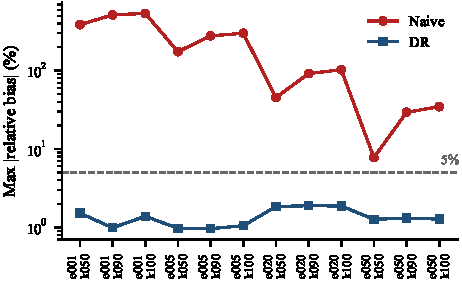
\includegraphics[width=\columnwidth]{figures/sweep_bias.pdf}
\caption{Maximum absolute relative bias across the 12 observation-rate cells, log scale. The dashed line is 5\%. Naive bias is 7.8--538.5\%; DR is at most 1.89\% in the mean.}
\label{fig:sweep}
\end{figure}

\begin{table}[t]
\centering
\caption{Observation-rate sweep. Naive is the maximum across the four policies; DR is the mean. Cells are ordered by $e_{\text{approve}}$ then $\kappa_{\text{review}}$.}
\label{tab:sweep}
\footnotesize
\begin{tabular}{lrrrr}
\toprule
Cell & Naive & DR & Cov. & DR $P$(best)\\
\midrule
e001\_k050 & 386.5\% & 1.52\% & 85.5\% & 64\%\\
e001\_k090 & 515.5\% & 0.99\% & 84.5\% & 64\%\\
e001\_k100 & 538.5\% & 1.38\% & 85.0\% & 64\%\\
e005\_k050 & 174.6\% & 0.97\% & 95.0\% & 68\%\\
e005\_k090 & 278.5\% & 0.96\% & 95.5\% & 68\%\\
e005\_k100 & 300.1\% & 1.05\% & 95.5\% & 68\%\\
e020\_k050 & 45.3\% & 1.84\% & 94.0\% & 76\%\\
e020\_k090 & 91.8\% & 1.89\% & 94.0\% & 80\%\\
e020\_k100 & 102.7\% & 1.87\% & 94.0\% & 80\%\\
e050\_k050 & 7.8\% & 1.26\% & 95.5\% & 96\%\\
e050\_k090 & 29.4\% & 1.31\% & 96.0\% & 100\%\\
e050\_k100 & 34.7\% & 1.27\% & 96.0\% & 100\%\\
\bottomrule
\end{tabular}
\end{table}

\subsection{Cost sensitivity and the ranking counterexample}
The ranking result is not universal. At a false-reject cost of 0.50 (\texttt{frej\_050}, 50 replications), the naive rule selects the true best policy \textbf{100\%} of the time while DR selects it \textbf{58\%}. The naive point estimate is still badly biased (+162.7\% to +291.2\%, coverage 0\%), so this is not a case where naive is accurate; it is a case where a biased point estimate preserves the ranking and an accurate point estimate does not. At 0.02 (\texttt{frej\_002}), naive is 64\% and DR 68\%; in the main scenario, naive is 0\% and DR 72\%. A post-hoc action-weighted Hájek baseline (50 replications) has a maximum relative bias of \textbf{2.9\%} in the main scenario and \textbf{2.4\%} at \texttt{frej\_050}, but selects the true best policy only \textbf{62\%} and \textbf{58\%} of the time. The naive point-estimate gap is therefore not merely an unweighted-mean artifact; the ranking effect survives a more realistic baseline. The practical rule is to report the cost curve and both metrics, not to claim that the correction always ranks better.

\subsection{Estimated and covariate propensities}
With estimated action-level propensities, DR is at 1.43\% and 93.5\% coverage; IPW is at 2.92\% and 92.0\%. Both survive action-level estimation; DR is better under noise (at $\sigma=0.25$, DR 1.58\% and IPW 7.01\%). Under covariate-dependent observation, action-level IPW fails (67.52\% bias, 1.0\% coverage) and action-level DR is better but still fails (21.25\%, 72.5\%). A fitted per-action covariate propensity model recovers the oracle: IPW 1.97\% and DR 2.48\% without delay; 3.35\% and 3.68\% with the 45-day delay. The practical rule is to match the propensity model to the observation mechanism and report the weight diagnostics.

\subsection{Double robustness}
Fig.~\ref{fig:dr} reports the known-truth test. With the correct propensity and a wrong outcome model (main effects only, missing an interaction), the plug-in is biased by 5.09\%, IPW by 0.69\%, and DR by 0.14\%. With a wrong propensity (1.6$\times$) and the correct outcome model, the plug-in is at 0.34\%, IPW at $-36.72$\%, and DR at 0.36\%. When both are wrong, DR is at 2.09\%, so the property is a safety net, not a guarantee.

\begin{figure}[t]
\centering
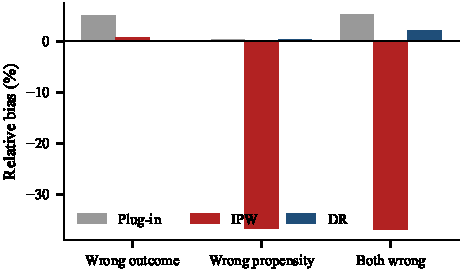
\includegraphics[width=\columnwidth]{figures/double_robustness.pdf}
\caption{Double-robustness test. DR stays near zero when either nuisance is correct; IPW fails with a wrong propensity and the plug-in fails with a wrong outcome model.}
\label{fig:dr}
\end{figure}

\subsection{Bounds and the F5 gate}
The main-scenario bounds interval is 0.009942; with a low false-reject cost (\texttt{frej\_002}), it is 0.203, twenty times wider. The narrow interval covers the true full-population value in 34\% of replications and passes the pre-registered 90\% gate in only 15 of 88 policy--scenario cells. The widened interval passes in 77 of 88 cells; the 11 failures are exactly the cells where the \Pzero\ estimate is biased (outcome-dependent labels, action-level covariate misspecification, and the 90-day delay). The correct reading is that the narrow interval is not a confidence interval, and the widened interval is valid but four times wider.

\subsection{Temporal stability}
Re-running the main scenario on months 5 and 6 separately gives naive biases of 230.4\% and 255.0\%, DR biases of 0.89\% and 0.43\%, DR coverage of 94.0\% and 91.0\%, and naive $P(\text{best})$ of 0\% in both months (DR 65\% and 63\%). The sign and the ranking conclusion hold; the exact percentage does not. This is a within-dataset stability check, not external validity.

\subsection{Case study}
The case study is a 20,000-row synthetic log with a 5\% review capacity, 8.9\% approve labels, and a candidate score that is an \emph{oracle}: a less noisy estimate of the true fraud probability, not a model trained on pre-decision features. The naive backtest says the candidate is 6.3\% more expensive; the true \Pzero\ cost is 12.4\% lower. The report returns a difference of $-0.0859$ with a 95\% interval $[-0.1640,-0.0077]$, $P(\text{candidate cheaper})=0.984$, and an expected regret of 0.0002 for the candidate versus 0.0861 for the incumbent. It recommends the candidate. Fig.~\ref{fig:case} shows the flip.

\begin{figure}[t]
\centering
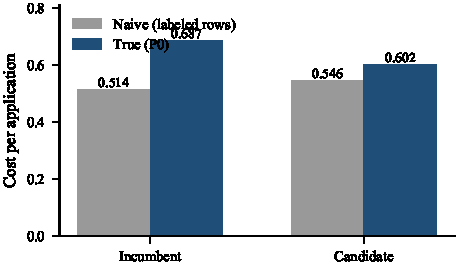
\includegraphics[width=\columnwidth]{figures/case_study.pdf}
\caption{Case study. The naive labeled mean ranks the candidate worse; the true \Pzero\ cost ranks it better. The report returns $P(\text{candidate cheaper})=0.984$.}
\label{fig:case}
\end{figure}

\section{Discussion}

\subsection{What the evidence supports}
The evidence supports four statements. First, under selective and delayed observation, the naive labeled mean is biased and can reverse the policy ranking; the direction and magnitude are conditional on the observation rates, and the ranking is also cost-dependent (at \texttt{frej\_050}, naive ranks correctly while DR does not). Second, DR recovers the \Pzero\ value when the propensity is known, and it is approximately unbiased when either the propensity or the outcome model is correct. Third, the ranking is a separate quantity: at the lowest label rate, DR's point estimate is accurate but its probability of selecting the true best policy is 64\%. Fourth, the reject margin is not point-identified; the narrow bounds fail their coverage gate, and the widened interval is valid but wide.

\subsection{Practical rules}
The results suggest five rules for a risk team. (i) Report the \Pzero\ value and the reject bounds separately; never present the \Pzero\ number as the full-policy value. (ii) Declare the observation mechanism; an outcome-dependent mechanism should refuse an action-only estimate. (iii) Match the propensity model to the mechanism; action-level weighting fails when observation depends on application features. (iv) Report the ranking metric, not only the point estimate. (v) Size the audit for the decision: a 5\% difference can require tens of thousands of labels, and the report should say so before the pilot. (vi) Never present a \Pzero\ recommendation as a full-policy decision; report the full-policy difference bound and, when it includes zero, the break-even rejected-fraud rate.

\subsection{Limitations}
The evidence is a simulation on one public synthetic dataset with a normalized cost matrix. The observation mechanism is chosen, not measured. There is no partner log and no independent validator, so the production claim is not established. The candidate-vs-incumbent interval treats the outcome model and propensity as fixed; a refitting bootstrap would be more honest. The audit-only estimate is post-stratified by follow-up time, with a within-stratum missing-at-random assumption. It targets the logging-approved population, not the candidate's approved population; a candidate that changes who is approved needs a candidate-specific audit. The reject margin remains a design problem: a controlled approval design or an explicit assumption is needed, not a better estimator.

\subsection{Regulatory relevance}
The measurement discipline is close to what model-risk guidance asks for: a stated estimand, documented assumptions, independent validation, stress testing, and monitoring \cite{bsp1213,bspsapiens}. The paper does not claim compliance; it provides an artifact a validator can inspect.

\section{Conclusion}
Account-opening fraud policies are evaluated on data the incumbent policy selected. This paper separates the identified \Pzero\ value from the unidentified reject margin, gates the estimate, and tests the estimator under the failure modes that matter: sparse and delayed labels, estimated propensities, covariate-dependent observation, outcome-dependent labels, and model misspecification. The result is a measurement layer that is useful precisely because it refuses to answer when the log cannot support the answer. The next step is a partner pilot with a real log and an independent validator.

\bibliographystyle{IEEEtran}
\bibliography{references}

\end{document}
